\documentclass[tikz, border=5mm]{standalone}

\usetikzlibrary{arrows.meta,decorations.markings,fit,calc, positioning}

\definecolor{componentColor}{RGB}{210,210,210}
\definecolor{systemColor}{RGB}{230,230,230}

\tikzset{component/.append style={fill=componentColor, align=center, draw, minimum width=2cm, minimum height=1.5cm, rounded corners=.3cm}}
\tikzset{system/.style={component, fill=systemColor, rounded corners=0cm}}

\tikzstyle{arrow} = [-{Latex[scale=3.0]}]
\tikzset{arrowLabel/.append style={minimum height=.25cm, draw=none}}
\begin{document}

	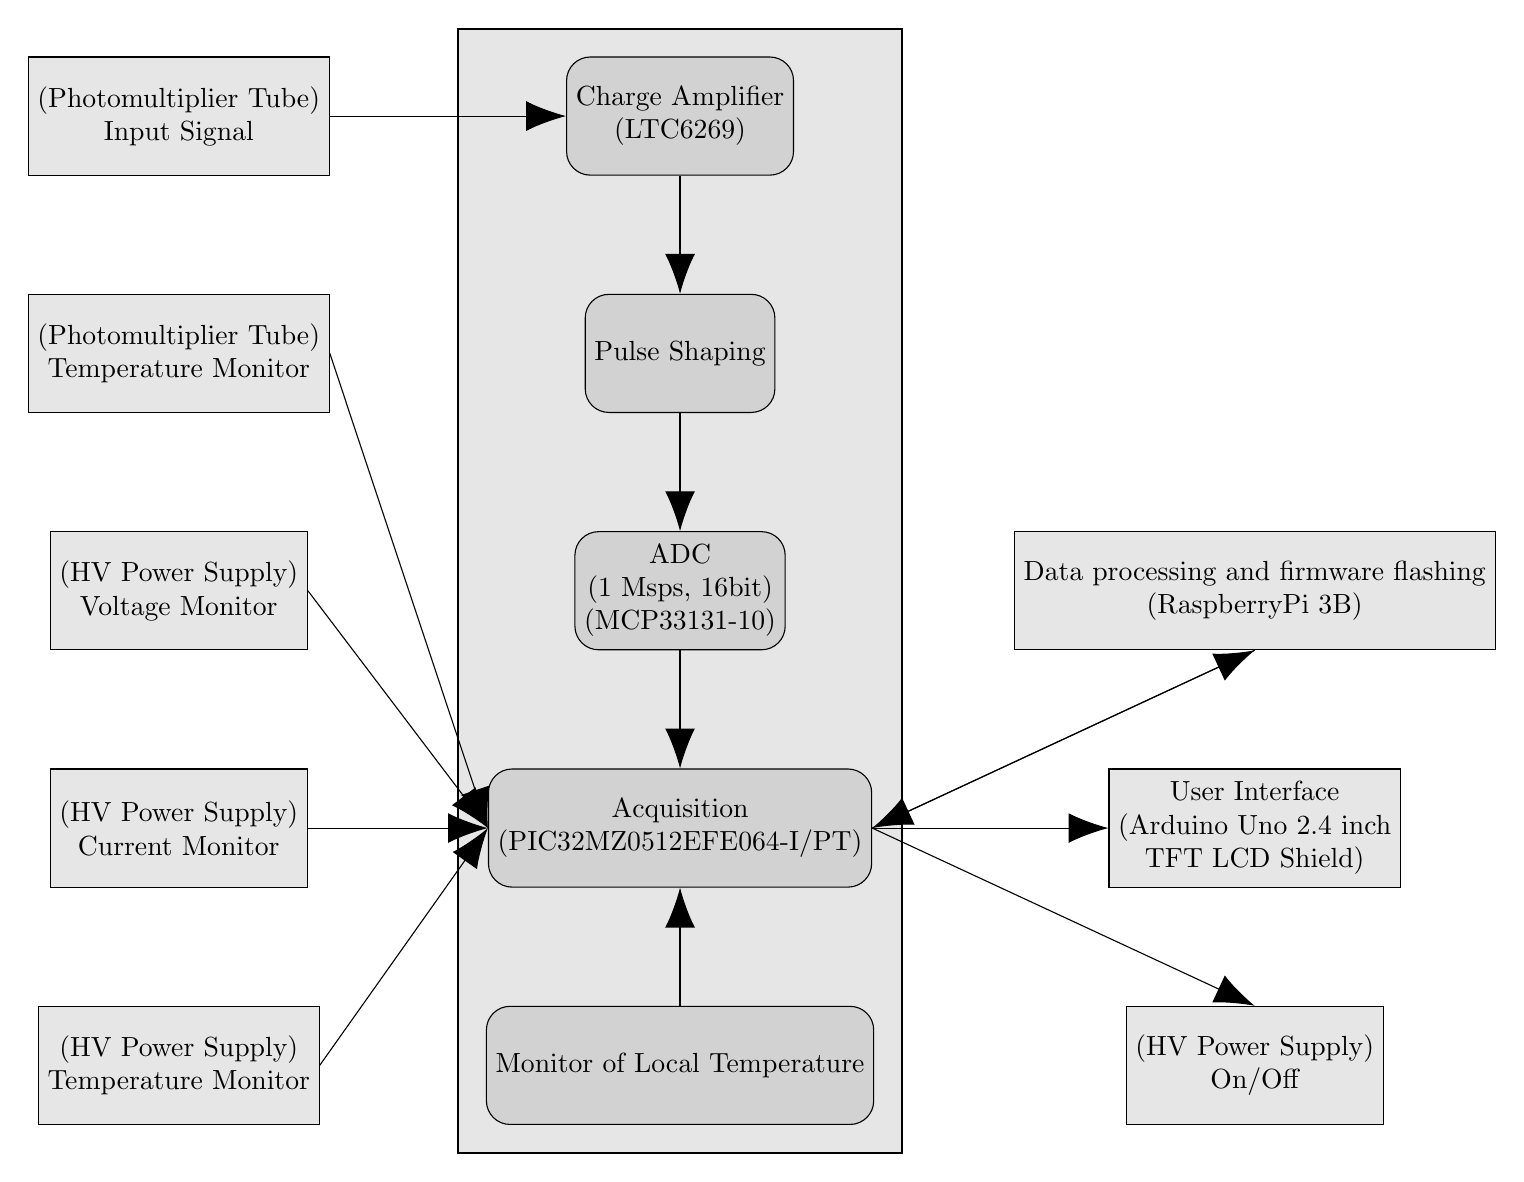
\begin{tikzpicture}[node distance=1.5cm and 3cm]
	% Nodes
	\pgfdeclarelayer{background}
	\pgfsetlayers{background,main}
	
        \node (photomultiplier) [system] {(Photomultiplier Tube)\\ Input Signal};		
		\node (photomultipliertemperature) [system, below=of photomultiplier] {(Photomultiplier Tube)\\ Temperature Monitor};		
		\node (hvvoltage) [system, below=of photomultipliertemperature] {(HV Power Supply)\\ Voltage Monitor};	
		\node (hvcurrent) [system, below=of hvvoltage] {(HV Power Supply)\\ Current Monitor};	
		\node (hvtemperature) [system, below=of hvcurrent] {(HV Power Supply)\\ Temperature Monitor};	

        \node (amplifier) [component, right=of photomultiplier] {Charge Amplifier\\ (LTC6269)};	
		\node (pulseshaping) [component, below=of amplifier] {Pulse Shaping};	
		\node (adc) [component, below=of pulseshaping] {ADC\\ (1 Msps, 16bit)\\ (MCP33131-10)};	
		\node (acquisition) [component, below=of adc] {Acquisition \\ (PIC32MZ0512EFE064-I/PT)};	
		\node (temperaturemonitor) [component, below=of acquisition] {Monitor of Local Temperature};	
	
		\node (gui) [system, right=of acquisition] {User Interface\\ (Arduino Uno 2.4 inch \\ TFT LCD Shield)};	
		\node (pi) [system, above=of gui] {Data processing and firmware flashing\\ (RaspberryPi 3B)};
		\node (hvonoff) [system, below=of gui] {(HV Power Supply)\\ On/Off};

		\begin{pgfonlayer}{background}
		\node[system, draw, thick, inner xsep=1em, inner ysep=1em, fit= (amplifier) (pulseshaping) (adc) (acquisition) (temperaturemonitor)] {};
		\end{pgfonlayer}
	    
		% Connectors
		\begin{scope}[->]
		
		\draw [arrow] (photomultiplier) -- (amplifier);
		\draw [arrow] (amplifier) -- (pulseshaping);
		\draw [arrow] (pulseshaping) -- (adc);
		\draw [arrow] (adc) -- (acquisition);
		\draw [arrow] (temperaturemonitor) -- (acquisition);

		\draw [arrow] (photomultipliertemperature.east) -- (acquisition.west);
		\draw [arrow] (hvcurrent) -- (acquisition);
		\draw [arrow] (hvvoltage.east) -- (acquisition.west);
		\draw [arrow] (hvtemperature.east) -- (acquisition.west);

		\draw [arrow] (acquisition) -- (gui);
		\draw [arrow] (acquisition.east) --  (pi.south);
		\draw [arrow] (pi.south) -- (acquisition.east);
		\draw [arrow] (acquisition.east) --  (hvonoff.north);


	\end{scope}

\end{tikzpicture}
\end{document}